\documentclass[10pt]{beamer}

\usetheme[progressbar=frametitle]{metropolis}
\usepackage{appendixnumberbeamer}

\usepackage{booktabs}
\usepackage[scale=2]{ccicons}
\usepackage{pgfplots}
\usepgfplotslibrary{dateplot}
\usepackage{xspace}
\newcommand{\themename}{\textbf{\textsc{metropolis}}\xspace}

\usepackage[portuguese]{babel}
\usepackage[utf8]{inputenc}
\usepackage[authoryear]{natbib}
\usepackage{amsfonts, amsmath, amssymb, amsthm, thmtools}
\usepackage{graphicx}
\graphicspath{{figures/}{../figures/}}
\usepackage{caption,subcaption}

\usepackage{tikz}
\def\checkmark{\tikz\fill[scale=0.4](0,.35) -- (.25,0) -- (1,.7) -- (.25,.15) -- cycle;} 

\def\P{{\mathbb P}}
\def\E{{\mathbb E}}
\def\I{{\mathbb I}}
\def\L{{\mathcal L}}
\def\D{\mathcal{D}}
\def\G{{\mathbb G}}
\def\U{{\mathbb U}}
\def\F{\mathbb{F}}
\def\FF{\mathcal{F}}

\title{Statistical analysis of AMPARO's data}
% \date{\today}
\date{}
\author{Rafael Bassi Stern}
\institute{Federal University of São Carlos}
% \titlegraphic{\hfill\includegraphics[height=1.5cm]{logo.pdf}}

\begin{document}

\maketitle

\begin{frame}{}
 \setbeamertemplate{section in toc}[sections numbered]
 \tableofcontents[hideallsubsections]
\end{frame}

\section{A description of the game}

\begin{frame}{The goalkeeper's game}
 The game was applied to patients with 
 Parkinson's disease and
 a control group.
 \metroset{block=fill}
 \begin{exampleblock}{Steps}
  \begin{itemize}
   \item Select a direction between: left, center or right.
	 \item Algorithm determines correct direction.
 	 \item Iterate.
 	\item Each stage uses a different algorithm.
  \end{itemize}
 \end{exampleblock}
\end{frame}

\begin{frame}{The goalkeeper's game}
 \metroset{block=fill}
 \begin{exampleblock}{Stages}
  \begin{itemize} 
   \item Warming-up
	 \item Deterministic with hints
	 \item Deterministic without hints
	 \item \ldots
	 \item Memory game
  \end{itemize}
 \end{exampleblock}
 Each stage was designed to capture
 a specific type of information.
\end{frame}

\begin{frame}{The goalkeeper's game}
 \metroset{block=fill}
 \begin{alertblock}{Initial goals}
  \begin{itemize} 
   \item Validate the information obtained from the game.
	 \item Predict variables related to Parkinson's disease
	 using the goalkeeper's game.
  \end{itemize}
 \end{alertblock}
 \begin{alertblock}{Challenge}
  \begin{itemize} 
   \item High dimensional features and small sample size.
  \end{itemize}
 \end{alertblock}
\end{frame}

\section{A model for learning}

\begin{frame}{The data}
 \metroset{block=fill}
 \begin{exampleblock}{Data description}
  \begin{itemize} 
   \item $i$: the stage of the game, $i \in \{1,2,3,4\}$.
	 \item $j$: and id for each patient, $1 \leq j \leq 67$.
	 \item $k$: a turn number.
	 \item $X_{i,j,k}$: the indicator that patient $j$
	 chose the right answer in the $k$-th turn of
	 the $i$-th stage of the game,
	 $X_{i,j,k} \in \{0,1\}$.
	 \item $Y_{i,j,k}$: the time spent by patient $j$
	 in the $k$-th turn of the $i$-th stage of the game,
	 $Y_{i,j,k} \in \mathbb{R}^+$.
	 \item $S_{i}$: level of schooling of patient $i$.
  \end{itemize}
 \end{exampleblock}
\end{frame}

\begin{frame}{The data}
 \metroset{block=fill}
 \begin{alertblock}{Challenge}
  \begin{itemize}
   \item $n=67$.
	 \item Covariates: $8$ time series per patient.
	 \item $S_{i}$ is very correlated with predicted variables.
	\end{itemize}
 \end{alertblock}
\end{frame}

\begin{frame}{A model for learning}
 \metroset{block=fill}
 \begin{exampleblock}{Statistical model}
  \begin{align*}
	 g(s) 
	 &= \frac{\exp(s)}{1+\exp(s)} \\
	 \P(X_{i,j,k}=1)
	 &= \gamma_{i,j} \cdot g(-\log(3\gamma_{i,j})+\alpha(S_{i})+k \cdot \beta_{i,j})
	\end{align*}
 \end{exampleblock}
 \begin{alertblock}{Strategy}
  \begin{itemize}
   \item Data might lie on a low dimensional manifold.
	 \item Use estimated parameters as covariates.
	\end{itemize}
 \end{alertblock}
\end{frame}

\begin{frame}{A model for learning}
 \begin{figure}
  \centering
  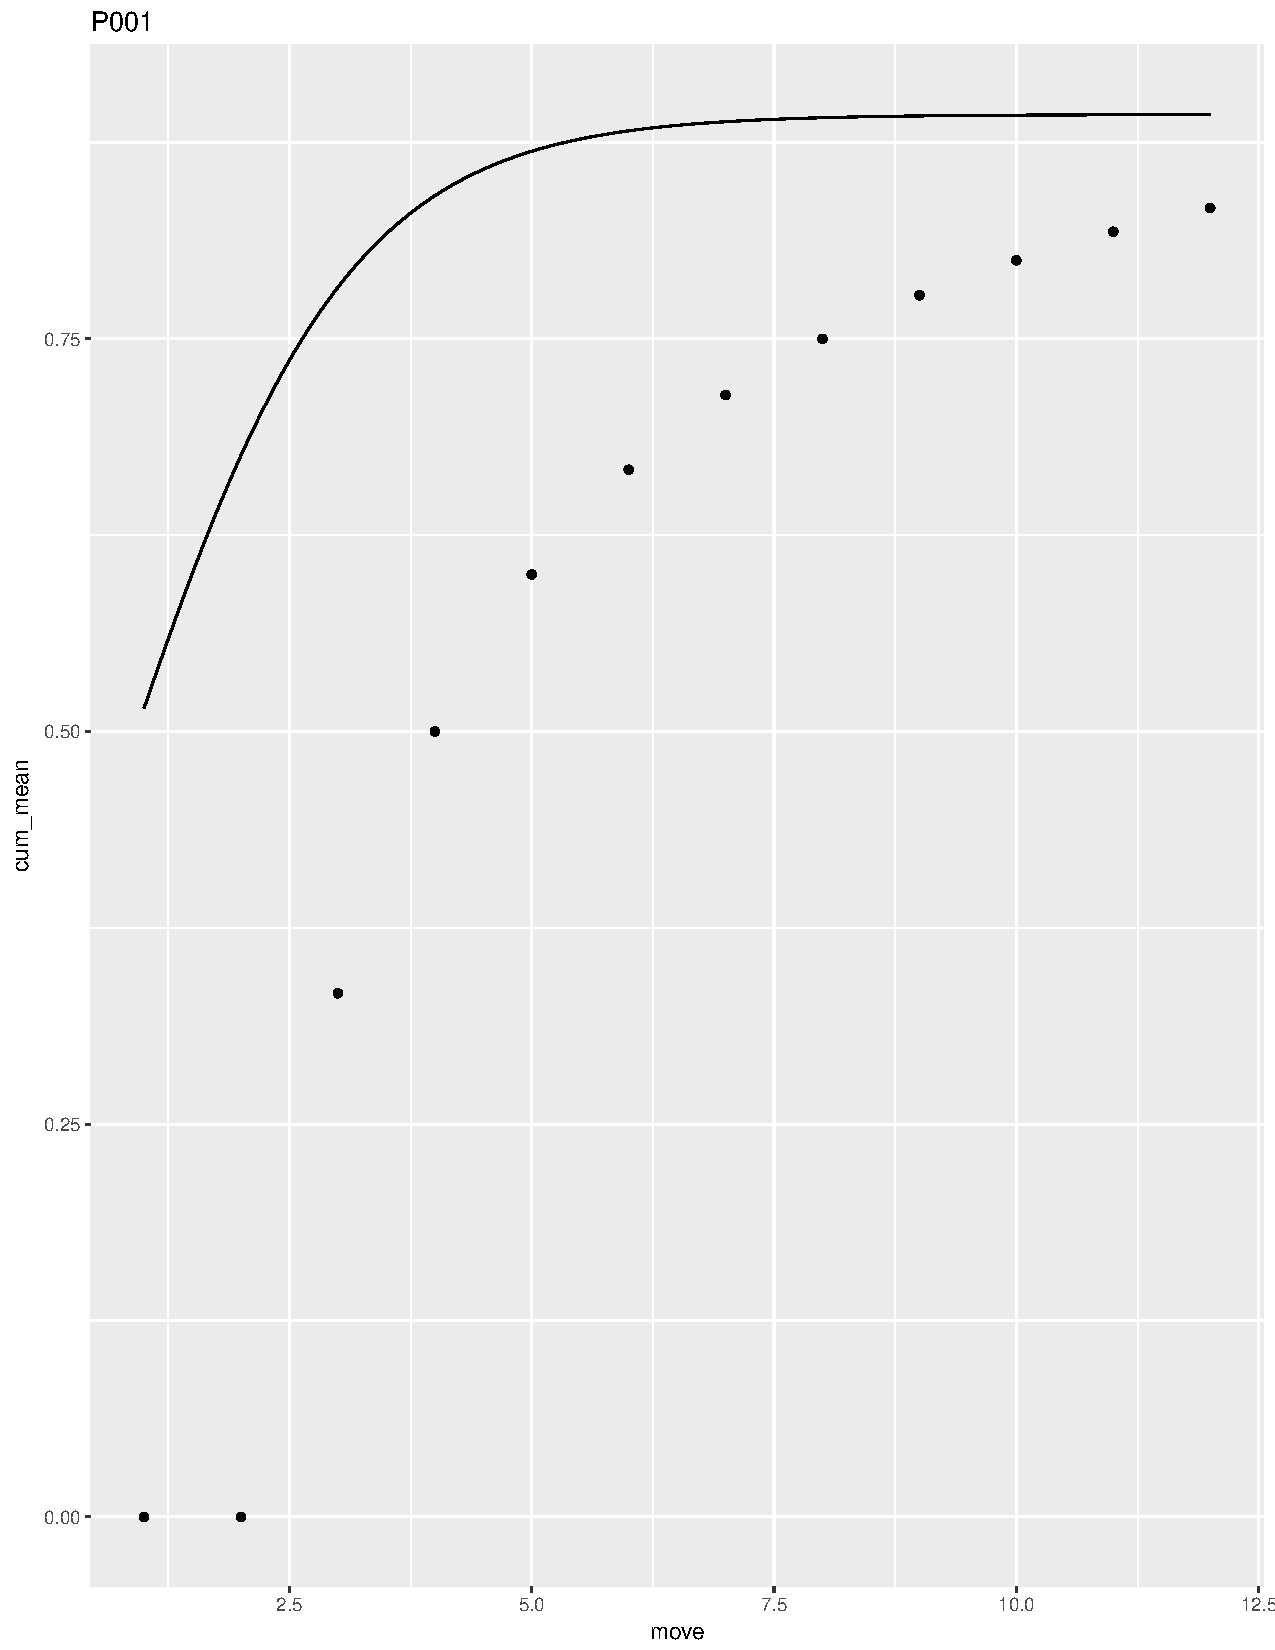
\includegraphics[scale=0.25]{exemplo-modelo}
 \end{figure}
\end{frame}

\begin{frame}{Fitting the model}
 \metroset{block=fill}
 \begin{alertblock}{Challenge}
  \begin{itemize}
   \item Obtain sparse parameter estimation.
	 \item No analytical solution.
	\end{itemize}
 \end{alertblock}
 \begin{exampleblock}{Solution}
  \begin{itemize}
   \item Bayesian estimation with sparse priors.
	 \item Posterior calculation via HMC (Stan).
	\end{itemize}
 \end{exampleblock}
\end{frame}

\section{Building classifiers}

\begin{frame}{Response variables}
 \metroset{block=fill}
 \begin{exampleblock}{Types}
  \begin{itemize}
	 \item MoCA: Montreal Cognitive Assessment.
	 \item UPDRS III: Unified Parkinson's Disease Rating Scale.
	 \item BEST: Balance Evaluation Scale Test.
	\end{itemize}
 \end{exampleblock}
 Each variable type has several instances.
\end{frame}

\begin{frame}{Logistic regression based on goalkeeper's game}
 \begin{table}
  \begin{tabular}{l|lll}
	 \hline
	 response    & baseline & accuracy & golden standard (moca) \\
	 \hline
	 updrs tot   & 0.54     & 0.66 & 0.72 \\
	 updrs rig   & 0.52     & 0.65 & 0.73 \\
	 best reat   & 0.52     & 0.66 & 0.72 \\
	 best rest   & 0.5      & 0.66 & 0.72 \\
	 moca evoc   & 0.5      & 0.69 & 0.8  \\
	 best lim    & 0.57     & 0.75 & 0.75 \\
	 best trans  & 0.5      & 0.7  & 0.74 \\
	 moca vis    & 0.56     & 0.77 & 0.83 \\
	 moca tot    & 0.52     & 0.72 & -    \\
	 best tot    & 0.5      & 0.72 & 0.72 \\
	 best march  & 0.5      & 0.75 & 0.73 \\
	 \hline
	\end{tabular}
 \end{table}
\end{frame}

\begin{frame}[allowframebreaks]{}
\bibliography{goalkeeper-validation}
\bibliographystyle{plainnat}
\end{frame}

\appendix

\end{document}
